% A Preliminary Literature Review which indicates: 
% (i) that you have studied the work of the major authors in your research field 
% (ii) that you are familiar with the major themes relevant to that subject area 
% (iii) what further investigations you intend to pursue as part of this dissertation. 
% You should bear in mind that you are reviewing the literature in order to develop sharper, 
% more insightful and focused research questions about your topic. 
% Therefore, your literature review should lead to and justify your research objectives and questions.

\xchapter{Fundamentação Teórica}
{Este capítulo apresenta conceitos necessários para a compreensão do trabalho.}
\label{fundamentacao}

A análise estática de código-fonte é o primeiro passo para coletar informações
necessárias em diversas atividades de verificação, medição e melhoria da
qualidade de produtos de software \cite{Cruz2009} \cite{Kirkov2010}. Ela é
realizada com base no código-fonte de um programa ou sistema de software, e a
partir daí descobre problemas e propriedades de sua qualidade estrutural
\cite{Chess2007}.

Ferramentas de análise estática estão disponíveis há décadas, em especial,
para programadores. A ferramenta Lint \cite{Johnson1978}, considerada a
primeira ferramenta de análise estática \cite{Gosain2015}, foi criada para
examinar programas escritos em linguagem C e aplicar regras de tipagem mais
estritas do que as regras dos próprios compiladores da linguagem.

Neste trabalho o nosso interesse reside em compreender características de
qualidade interna de ferramentas deste domínio de aplicação, do ponto
de vista de desenvolvedores interessados em manter e evoluir tais ferramentas
melhorando seus atributos de qualidade interna.

A seção \ref{analise-estatica} apresenta uma definição geral da análise
estática de código-fonte, suas aplicações, sua anatomia, seus formatos de
representação intermediária e técnicas mais comuns. A seção \ref{metricas} traz uma
definição de métricas de software e apresenta um conjunto de métricas
utilizados neste estudo, trazendo detalhes sobre métricas de complexidade
estrutural.

\section{Análise estática de código-fonte} \label{analise-estatica}

Análise estática de código-fonte é tem como objetivo prover
informações acerca de um programa a partir do seu código-fonte sem
necessidade de execução, e sem requerer qualquer outro artefato do programa
além do próprio código.

É um ramo que possui muitas das suas abordagens em comum com os estudos da
área de análise de programas ({\it program analysis}), especialmente na área de
compiladores, onde atua especialmente nas primeiras etapas do processo de compilação.

A análise estática de código-fonte é considerada uma atividade meio com
objetivo de suportar uma variedade de tarefas comuns da engenharia de
software; muitas dessas tarefas são substancialmente úteis em atividades de
manutenção. \citeonline{Binkley2007} define uma extensa lista dessas
atividades, incluindo:

\begin{multicols}{2}
  \begin{itemize}
    \item Análise de performance
    \item Compreensão de programas
    \item Desenvolvimento baseado em modelos
    \item Detecção de clones
    \item Evolução de software
    \item Garantia de qualidade
    \item Localizaçao de falhas
    \item Manutenção de software
    \item Recuperação arquitetural
    \item Testes
  \end{itemize}
\end{multicols}

Seja em qual atividade for, a análise estática possui uma importância
significativa, pois ao ser capaz de extrair informações diretamente do
código-fonte de um programa, pode auxiliar a responder perguntas necessárias
para as diversas atividades de desenvolvimento e evolução de software. Esta
importância se torna ainda mais aparente diante da ``lei'' da tendência para
execução \cite{Harman2010} que indica que todos os tipos de notação tem a
tendência de se tornar executáveis.

\subsection{Usos da análise estática de código-fonte} \label{usos}

A análise de programas trata, de modo geral, da descoberta de problemas e
fatos sobre programas, ela pode ser realizada sem a necessidade de executar o
programa (análise estática) ou com informações provenientes de sua execução
(análise dinâmica).

A idéia de que programas de computador podem ser utilizados para analisar
código-fonte de outros programas tem uma história de mais de 40 anos.  O
programa PFORT \cite{Ryder1974} foi projetado para localizar potenciais
problemas na portabilidade de código Fortran; em função da diversidade de
dialetos de Fortran, uma compilação sem erros não indicava que o programa
estava correto segundo os padrões da linguagem \cite{Wichmann1995}.

Desde então, ferramentas de análise estática de código-fonte têm surgido para
os mais diversos fins -- muitas delas a partir das pesquisas e
desenvolvimentos da área de compiladores.  O {\it parser} utilizado nessas
ferramentas têm funcionalidades análogas aos analisadores usados em
compiladores \cite{Anderson2008}.

O uso de tais ferramentas tem se
tornado mais e mais comum no ciclo de desenvolvimento de
software, sendo aplicadas em uma infinidade de atividades distintas visto que o
campo de aplicação destas ferramentas é bastante variado, cobrindo diferentes
objetivos. Dentre as atividades em que a análise estática de código-fonte é
usada \cite{Chess2007}, destacam-se:

\begin{description}

  \item \textit{Verificação de tipos}. 
    A forma mais amplamente utilizada de análise estática, e uma das quais os
    programadores estão mais familiarizados, é a checagem de tipo.
    Programadores dão pouca atenção a isto, visto que as regras são definidas
    pela linguagem de programação e executadas pelo próprio compilador, de
    forma que não se torna necessário entender como a análise acontece.  No
    entanto, esta atividade de verificação é análise estática e elimina toda
    uma categoria de erros de programação. Por exemplo, previne que
    programadores acidentalmente atribuam valores de forma incorreta a
    variáveis.  Ainda, ao capturar erros em tempo de compilação, esta checagem
    de tipo previne erros em tempo de execução.

  \item \textit{Verificação de estilo}. 
    Os verificadores de estilo são um tipo de análise estática que aplicam regras
    de forma mais superficial do que os verificadores de tipo. São regras
    relacionadas a espaços em branco, nomes, funções depreciadas, comentários,
    estrutura do programa, entre outros.  A maioria dos verificadores de
    estilo costumam ser bem flexíveis quanto ao conjunto de regras que aplicam
    uma vez que os programadores costumam ser bastante apegados aos seus
    próprios estilos de programação. Os erros reportados por verificadores de
    estilo são aqueles que afetam a leitura e a manutenabilidade do
    código-fonte, não indicando potenciais erros em tempo de execução como
    fariam os verificadores de tipo.

  \item \textit{Compreensão de programas}. 
    Ferramentas de compreensão de programa ajudam programadores a terem uma visão
    clara frente a grandes programas de computador, ou seja, programas com
    alto volume de código-fonte. Ambientes de desenvolvimento integrados (IDE)
    geralmente incluem funcionalidade de compreensão, por exemplo, ``encontrar
    todos os usos de um certo método'' ou ``encontrar a declaração de uma
    variável global''. Análises mais avançadas chegam a incluir, por exemplo,
    refatoração automática. Estas ferramentas de compreensão também são úteis
    para programadores interessados em entender código-fonte escrito por
    outros programadores.

  \item \textit{Verificação de programas}.
    Ferramentas de verificação de programa aceitam como entrada uma especificação
    e um conjunto de código-fonte e tenta provar que o código está deacordo
    com a especificação. Quando a especificação é uma descrição completa de
    todo o programa, a ferramenta de verificação poderá realizar uma checagem
    de equivalência para garantir que o código-fonte e a especificação
    combinam de forma exata. Programadores raramente têm acesso a uma
    especificação detalhada suficientemente para ser usada numa checagem de
    equivalência, o trabalho de criar esta especificação pode ser maior do que
    o trabalho de escrever o próprio código-fonte do programa, desta forma
    este tipo de verificação formal raramente acontece. Sendo mais comum a
    verificação em relação a uma especificação parcial que detalha apenas
    parte do comportamento do programa. Isto costuma ser chamado de
    verificação de propriedade, grande parte das ferramentas de verificação de
    propriedade funcionam aplicando inferências lógicas ou verificação de
    modelos.

  \item \textit{Localização de bugs}. 
    O propósito de uma ferramenta de localização de bugs não está em questões de
    formatação, como é a verificação de estilo, nem em realizar uma exaustiva
    e completa comparação contra uma especificação, como uma ferramenta de
    verificacao de programa. Ao invés disso, um localizador de bugs está
    preocupado em apontar locais onde o programa, possivelmente, irá se
    comportar de forma inesperada. A maioria das ferramentas de localização de
    bugs são fáceis de usar porque costumam vir com um conjunto de regras
    ({\it bug idioms}) para descrição de padrões de código que indicam bugs.
    Algumas destas ferramentas costumam usar os mesmos algoritmos utilizados
    por ferramentas de verificação de propriedade.

  \item \textit{Avaliação de segurança}. 
    Ferramentas de análise estática para segurança usam as mesmas técnicas
    encontradas nas outras ferramentas, mas por ter um propósito diferente,
    identificar problemas de segurança, aplicam estas técnicas de forma diferente.
    As primeiras ferramentas de segurança (ITS4, RATS, Flawfinder) eram pouco mais
    do que um {\it ``grep''} melhorado; na maior parte, elas escaneavam o código
    procurando por funções como por exemplo {\it ``strcpy()''} que são
    facilmente usadas de forma inadequada e devem ser inspecionadas
    manualmente no processo de revisão de código-fonte. A evolução deste tipo
    de ferramenta de segurança levou a técnicas híbridas de verificação de
    propriedade e de localização de bugs, de forma que muitas propriedades de
    segurança podem ser suscintamente expressas como propriedades de
    programas.

\end{description}

\subsection{Anatomia da análise de código-fonte} \label{anatomia}

Ferramentas de análise estática de código-fonte estão organizadas em partes ou
componentes, responsáveis por implementar três funções básicas \cite{Cruz2009}
\cite{Binkley2007}: a) extração de dados, b) geração de representação
intermediária, e c) análise. A ferramenta de análise de código-fonte
CodeSonar\footnote{https://www.grammatech.com/products/codesonar} segue tal
organização, conforme mostra a Figura \ref{static-analysis-representation}.

\begin{figure}[h]
  \center
  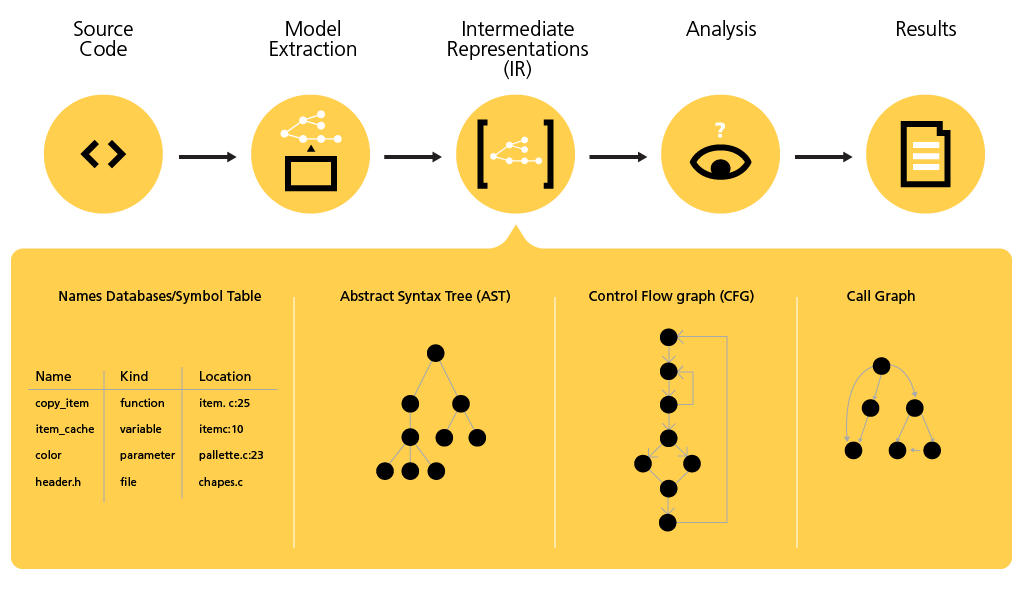
\includegraphics[scale=0.4]{imagens/static-analysis-representation.png}
  \caption{CodeSonar: Representação da Análise Estática \cite{GrammaTech2016}}
  \label{static-analysis-representation}
\end{figure}

\begin{description}

  \item \textit{Extração de dados}.
    O processo de recuperar dados para futuro processamento ou armazenamento é
    chamado de extração de dados. 

    O primeiro componente da análise de código-fonte é a extração de dados,
    responsável por ler o código-fonte do programa e gerar uma ou mais
    representações intermediárias. Em essência, este componente converte a sintaxe
    de um programa em uma outra sintaxe abstrata e mais adequada para análise
    posterior. Este componente é usualmente chamado de analisador sintático
    (ou {\it parser}) e apesar de teoricamente não ser uma tarefa difícil,
    apresenta enormes desafios diante da complexidade das linguagens de
    programação modernas.

  \item \textit{Representação intermediária}.
    Exportar os dados extraídos para uma representação intermediária é uma
    estratégia comum para facilitar análise e transformação de dados e
    possivelmente adição de metadados.

    Os dados obtidos na extração precisam ser representados em um formato mais
    abstrato. Esta é a responsabilidade do segundo componente da análise de
    código-fonte: armazenar os dados coletados usando uma representação
    intermediária em formato mais adequado para análise automática, abstraindo
    aspectos particulares do programa e da linguagem de programação.

    Alguns tipos de representação intermediária têm sua origem na área de
    compiladores; algumas delas são produzidas diretamente pelo {\it parser}
    enquanto outras requerem uma análise específica. Os formatos mais comuns
    são geralmente baseados em grafos. 

    Alguns formatos comumente utilizados são:
    \begin{multicols}{2}
      \begin{itemize}
        \item Árvore sintática abstrata
        \item Grafo de fluxo de controle
        \item Árvore sintática abstrata decorada
        \item Grafo de dependência de módulos
        \item Atribuição estática única
        \item Grafo de dependência de valores
      \end{itemize}
    \end{multicols}

    Estas representações podem ser utilizadas tanto na análise estática quanto
    na análise dinâmica. O uso de um ou outro formato depende do tipo de
    análise e seu propósito. Pode-se combinar diferentes tipos no sentido de
    enriquecer e estruturar a informação extraída.

  \item \textit{Análise}.
    Este componente é responsável por realizar inferências a partir dos dados
    representados internamente. O processo requer que as informações
    armazenadas estejam interconectadas e também interrelacionadas com
    conhecimento anterior. Esta análise pode gerar conhecimento quantitativo
    ou qualitativo, como, por exemplo, métricas de software ou mineração de
    dados, respectivamente. Técnicas de visualização podem ser usadas para
    apoiar este processo.

    Diversas técnicas foram desenvolvidas ao longo do tempo para realizar
    análise, algumas delas são brevemente descritas na seção \ref{tecnicas}.

\end{description}

\subsection{Formatos de representação intermediária} \label{formatos}

\cite{Zaytsev2015} autor enumera e descreve uma quantidade de grafos de
representação interna para programacao funcional.

Essencialmente, um formato de representação intermediária é uma abstração precisa
das propriedades de um programa representado em um domínio menor. Os
compiladores normalmente constroem esta representação a fim de possuir um
modelo do programa sendo compilado, é comum que compiladores utilizem diversos
formatos durante o curso da compilação.

Em ferramentas de análise estática estes formatos são utilizados durante a
fase de análise para cumprir diversos objetivos, como por exemplo, calcular
métricas de código-fonte. A métrica de complexidade ciclomática de McCabe
\cite{McCabe1976}, por exemplo, é definida com base no grafo de fluxo de controle (CFG) do
programa com o seguinte cálculo $CC = e - n + 2p$. Onde: {\bf e} é o número de
arestas; {\bf n} é o número de nós; e {\bf p} é o número de componentes
fortemente conectados no grafo CFG.

Assim, percebe-se que cada formato de representação intermediária \cite{Nielson2015}
\cite{Stanier2013} \cite{Cruz2009} \cite{Ramalho1996} pode ter fins e
objetivos bastante distintos, dentre os formatos mais comuns podemos destacar:

\begin{description}

  \item \textit{Árvore sintática abstrata}.
    A árvore sintática abstrata (AST - Abstract Syntax Tree) representa um
    programa tratando os elementos do código-fonte como operadores e
    operandos organizados em nós numa árvore, este formato de representação é
    muito popular em tradutores {\it
    source-to-source}\footnote{http://en.wikipedia.org/wiki/Source-to-source\_compiler}.

  \item \textit{Grafo de fluxo de controle}.
    O grafo de fluxo de controle (CFG - Control Flow Graph ou Call Graph) é um grafo direcionado
    representando a estrutura de controle de um programa e sua sequência de
    instruções, onde as arestas mostram os possíveis caminhos de execução. Este
    formato é amplamente utilizado em métodos formais para otimização de
    código-fonte.

  \item \textit{Grafo de fluxo de dados}.
    O grafo de fluxo de dados (DFG - Data Flow Graph) é também um grafo
    direcionado onde as arestas representam o fluxo de dados entre as
    operações do programa, este formato pode ser visto como um companheiro do
    grafo de fluxo de controle (CFG) e pode ser gerado ao longo de uma mesma
    análise.

  \item \textit{Árvore sintática abstrata decorada}.
    Árvore sintática abstrata decorada (DAST - Decorated Abstract Syntax Tree) é
    uma árvore sintática abstrata (AST) melhorada através de um processo de
    definiçao de atributos para os símbolos do programa de forma declarativa
    com uso de uma Gramática de
    Atributos\footnote{https://en.wikipedia.org/wiki/Attribute\_grammar}.

  \item \textit{Grafo de dependência de módulos}.
    O grafo de dependência de módulos (MDG - Module Dependence Graph) é um grafo
    onde os módulos são representados como nós e as arestas representam as
    relacões entre eles, indicando dependência entre os mesmos.

  \item \textit{Atribuição estática única}.
    Atribuição estática única (SSA - Static Single Assignment) pode ser vista
    como uma variação ou uma propriedade de outros formatos de representação
    intermediária, é um método que faz cada variável ser atribuída apenas uma única
    vez, facilitando a descoberta de informaçoes sobre os dados representados.

  \item \textit{Grafo de dependência de valores}.
    O grafo de dependência de valores (VDG - Value Dependence Graph) é uma
    variação que melhora (ao menos para algumas análises) os resultados
    obtidos a partir da atribuição estática única (SSA). Ele representa tanto
    o fluxo de controle quanto o fluxo de dados e assim simplifica a análise.

\end{description}

\subsection{Técnicas de análise} \label{tecnicas}

Inúmeras técnicas e métodos distintos podem ser utilizados pelas ferramentas
de análise estática, seja com o objetivo de verificação de tipos, localização
de bugs, compreensão de programas, avaliação de segurança, ou outra finalidade
qualquer. Segundo \citeonline{German2003}, \citeonline{Li2010},
\citeonline{Hofer2010} as técnicas e métodos mais comumente encontrados nas
ferramentas atuais são:

\begin{description}

  \item \textit{Análise léxica}.
    A análise léxica é responsável por quebrar o programa em pequenos fragmentos
    (ou {\it tokens}) e verificar se estes fragmentos são palavras válidas
    para uma dada linguagem. A análise léxica não leva em consideração a
    sintaxe do programa, sua semântica ou a interação entre módulos.

  \item \textit{Combinação de padrões de texto}.
    A combinação de padrões de texto ({\it Text-based Pattern Matching}) é a
    maneira mais simples e rápida de procurar vulnerabilidades num código
    fonte.

  \item \textit{Inferência de tipos}.
    A inferência de tipos ({\it Type inference}) refere-se a identificar o
    tipo de variáveis e funções e avaliar se o acesso a elas está em
    conformidade com as regras da linguagem. Linguagens de programação com
    sistema de tipagem incluem mecanismos deste tipo de análise.

  \item \textit{Análise de fluxo de dados}.
    A análise de fluxo de dados ({\it Data flow analysis}) resume-se a coletar
    informação semântica do código-fonte do programa, e com métodos algébricos
    deduzir a definição e uso das variáveis em tempo de compilação. O objetivo
    é mostrar que nenhum caminho de execução do programa acessa uma variável
    sem definição ou atribuição prévia.

  \item \textit{Verificação de regra}.
    A verificação de regra ({\it Rule checking}) consiste em checar a segurança
    do programa através de um conjunto de regras pré-estabelecidas.

  \item \textit{Análise de restrição}.
    A análise de restrição ({\it Constraint analysis}) consiste em gerar
    e resolver restrições no processo de análise de um programa.

  \item \textit{Comparação caminho}.
    Comparação caminho ({\it Patch comparison}) inclui comparação de caminho de
    código-fonte e de código-binário e é usada principalmente para encontrar
    brechas de vulnerabilidade já ``conhecidas'' e previamente divulgadas por
    fornecedores e praticantes da indústria de software.

  \item \textit{Execução simbólica}.
    A execução simbólica ({\it Symbolic execution}) é usada para representar
    as entradas de um programa através do uso de valores simbólicos ao invés
    de dados reais, produz expressões algébricas sobre a entrada dos símbolos
    do programa durante o processo de implementação e pode detectar
    possibilidade de erros.

  \item \textit{Interpretação abstrata}.
    Interpretação abstrata ({\it Abstract interpretation}) é uma descrição
    formal da análise do programa. Pelo fato de apenas controlar atributos de
    programa de preocupaçao dos usuários, a interpretação da análise semântica
    é similar ao seu significado semântico real.

  \item \textit{Prova de teoremas}.
    Prova de teoremas ({\it Theorem proving}) é baseada na análise semântica do
    programa. Converte o programa em fórmulas lógicas e então tenta provar que
    o programa é um teorema válido usando regras e axiomas.

  \item \textit{Verificação de modelo}.
    O processo de verificação de modelos ({\it Model checking}) primeiro constrói
    um modelo formal do programa tal como uma máquina de estados ou um grafo
    direcionado, então examina e compara o modelo para verificar se o sistema
    cumpre as características pré-definidas. Esta técnica requer a definição e
    descrição das propriedades que devem ser verificados por um pedaço de
    software.

  \item \textit{Verificação formal}.
    Verificação formal ({\it Formal Checking} ou {\it Compliance Analysis}) é o
    processo de provar de forma automatizada que o código do programa está
    correto em relação a uma especificação formal dos seus requisitos.

  \item \textit{Análise de fluxo da informação}.
    Análise de fluxo da informação ({\it Information Flow Analysis}) identifica
    como a execução de uma unidade de código cria dependência entre entradas e
    saídas.

  \item \textit{Verificação de sintaxe}.
    Verificação de sintaxe ({\it Syntax Checks}) tem o objetivo de encontrar
    violação de regras tais como expressões mal-formadas ou fora do padrão.

  \item \textit{Verificação de intervalo}.
    A análise de verificação de intervalo ({\it Range Checking}) tem o objetivo
    de verificar que os valores dos dados permanecem dentro de intervalos
    especificados, bem como manter a precisão especificada.

\end{description}

%--------------------------------------%
\section{Métricas de software} \label{metricas}

No glossário de terminologia para engenharia de software do IEEE
\cite{ieee1990ieee}, a qualidade de software é definida como (1) o grau em que
um sistema, componente ou processo atende a requisitos especificados e (2) o
grau em que um sistema, componente ou processo atende às necessidades ou
expectativas de um usuário. 

Segundo o padrão para metodologia de qualidade de métricas de software do IEEE
\cite{software1998ieee}, uma métrica de qualidade de software é ``uma função
cujas entradas são dados de software e cuja saída é um valor numérico, que
pode ser interpretado como o grau em que um software possui um determinado
atributo que afeta sua qualidade''.

Métricas de software podem ser classificadas em métricas de processo, métricas
de projeto e métricas de produto.

Métricas de processo medem atributos relacionados ao ciclo de desenvolvimento
e manutenção de software. Métricas de projeto indicam se a execução do
processo está progredindo conforme planejado (por exemplo, relação entre o
tamanho do software entregue e o esforço total dispendido em seu
desenvolvimento).

Métricas de produto medem atributos de produtos e artefatos, como documentos,
diagramas, código-fonte e arquivos binários. Neste trabalho,
apenas métricas de produto serão utilizadas.

Métricas de produto podem ser classificadas em internas (medem propriedades
visíveis apenas aos desenvolvedores) ou externas (medem propriedades visíveis
aos usuários) \cite{Mohamed1994}.

Neste trabalho, são utilizadas métricas de produto e, especificamente,
métricas de código-fonte, que cobrem aspectos de tamanho, complexidade e
qualidade que podem ser medidos a partir do código-fonte de um software.

\subsection{Métricas de código-fonte} \label{metricas-de-codigo}

As propriedades visíveis aos desenvolvedores podem ser medidas através de
métricas de código-fonte. A observação e o monitoramento de seus valores podem
indicar aspectos relevantes à manutenibilidade de um programa. Dentre as
inúmeras métricas de código-fonte iremos destacar aquelas utilizadas no estudo
de \citeonline{Meirelles2013} onde associou-se características de qualidade de
produto de software à características de qualidade de código-fonte através da
observação de suas métricas, são elas:

\begin{itemize}
  \item {\bf ACC} {\it Afferent Connections per Class (Conexões aferentes de
    uma classe)}: mede a conectividade de uma classe através do número total de
    classes clientes, é definida pela seguinte fórmula:

\begin{equation}
\label{formula-acc}
ACC(C) = \sum_{i=1}^{n} cliente(Ci, C)
\end{equation}

Onde:

\begin{equation}
cliente(Ci, Cj) =
  \begin{cases}
    1 \text{ se } Ci \Rightarrow Cj \wedge Ci \neq Cj \\
    0 \text{ caso contrario} \\
  \end{cases}
\end{equation}

A notação $ Ci \Rightarrow Cj $ indica acesso à atributos, variáveis, métodos
ou funções entre módulos ou classes.

A métrica {\it Afferent Connections per Class} (Conexões aferentes de uma
classe) é encontrada na literatura com o nome {\it Afferent coupling}
(Acoplamento aferente) \cite{Martin1994}, o nome {\it Afferent Connections per
Class} (ACC) utilizado aqui foi introduzido no estudo de
\citeonline{Meirelles2010}, e por estarmos reproduzindo parte da abordagem
deste estudo adotaremos o mesmo nome.

A definição original da métrica não deixa claro exatamente o que compreende
dependencia entre classes, de forma que restam dúvidas sobre o que deve ser
contabilizado, a definição indica apenas que ``relacionamentos de classes''
devem ser considerados, como ``herança e associação'' por exemplo.

Apesar disso muitos autores \cite{Briand1999Unified, Fenton2014, Ferreira2008}
seguem a mesma definição da fórmula \ref{formula-acc}:
se uma classe A referencia outra classe B, então existe um acoplamento aferente
de B para A. Uma data classe A referencia outra classe B se (i) A chama um
método de B, (ii) A acessa um campo de B, ou (iii) A é uma subclasse de B.

É importante destacar que classes com um alto número de acoplamento aferente
desempenham um importante papel no sistema, porque erros ou modificações nestas
classes podem causar grande impacto em outras partes do sistema.

  \item {\bf ACCM} {\it Average Cyclomatic Complexity per Method (Média de
    complexidade ciclomática por método)}: mede a complexidade do programa
    \cite{McCabe1976}.

Essa métrica pode ser representada através de um grafo de fluxo de controle,
onde os nós representam uma ou mais instruções sequenciais e os arcos
orientados indicam o sentido do fluxo de controle entre várias instruções. A
complexidade ciclomática de um determinado grafo pode ser calculada através da
seguinte fórmula da teoria dos grafos:

\[ v(G) = e - n + 2 \]

Onde, $e$ é o número de arestas e $n$ é o número de nós do grafo.


  \item {\bf AMLOC} {\it Average Method LOC (Média do número de linhas de
    código por método)}: calcula o número médio de linhas de código por método
    de uma dada classe, indica se o código está bem distribuído entre os
    métodos, quanto maior, mais ``pesados'' são os métodos.

  \item {\bf ANPM} {\it Average Number of Parameters per Method (Média do
    Número de Parâmetros por Método)}: calcula a média de parâmetros dos
    métodos da classe \cite{Jagdish1997}. Computada calculando o número
    total de parametros de todos os métodos de uma classe dividido pelo número
    de métodos.

    Esta métrica é identificada na literatura apenas como NPM, aqui chamamos de
    ANPN para evitar conflito com a métrica {\bf NPM} {\it Number of Public
    Methods (Número de métodos públicos)}.

  \item {\bf CBO} {\it Coupling Between Objects (Acoplamento entre objetos)}:
    mede o acoplamento entre objetos do software \cite{Chidamber1994}
    calculando em nível de classe o número total de acessos à outras classes do
    mesmo sistema, é comum ser também chamada de Fan-out da classe. CBO é então
    definida pela seguinte fórmula:

\begin{equation}
\label{formula-cbo}
CBO(C) = \sum_{i=1}^{n} cliente(C, Ci)
\end{equation}

Onde:

\begin{equation}
cliente(Ci, Cj) =
  \begin{cases}
    1 \text{ se } Ci \Rightarrow Cj \wedge Ci \neq Cj \\
    0 \text{ caso contrario} \\
  \end{cases}
\end{equation}

A notação $ Ci \Rightarrow Cj $ indica acesso à atributos, variáveis, métodos ou funções
entre módulos ou classes.

Apesar de ser possível formalizar a métrica CBO através da fórmula acima, sua descriçao original é
bastante complexa, levando à implementações variadas do seu cálculo
\cite{Lincke2008}. A definição original, por exemplo, inclui explicitamente
acoplamento via herança \cite{Harrison1998}, no entando não deixa claro como
deve ser tratado métodos herdados \cite{Briand1999}. A definição original
afirma também que apenas chamadas explícitas (e não chamadas implicitas) de
construtores são contabilizadas. Algumas definições de CBO incluem não apenas $
cliente(Ci, Cj) $ mas também a recíproca $ cliente(Cj, Ci) $ de forma que o valor
final inclui classes que ela acessa somado ao número de classes do sistema que
a acessam \cite{Sant2008}.

Quanto mais as classes forem independentes, mais fácil é reutilizá-las e menos
arriscado é modificá-las. Classes mais acopladas precisam de mais rigor em
testes, pois mais partes do sistema dependem delas.

  \item {\bf DIT} {\it Depth of Inheritance Tree (Profundidade da árvore de
    herança)}: mede o número de ancestrais de uma classe \cite{Chidamber1994}.

É o número de superclasses ou classes ancestrais de uma dada classe. São
contabilizadas apenas as superclasses do sistema, ou seja, as classes de
bibliotecas externas não são contabilizadas. Nos casos onde herança múltipla é
permitida, considera-se o maior caminho da classe até uma das raízes da
hierarquia. Quanto maior for o valor DIT, maior é o número de atributos e
métodos herdados, e portanto maior é a complexidade.

%Os intervalos sugeridos
%são: até 2 (bom); entre 2 e 4 (regular); de 4 em diante (ruim). Entretanto,
%valores baixos indicam pouco reúso de código via herança.

  \item {\bf LCOM4} {\it Lack of Cohesion in Methods (Ausência de coesão em
    métodos)}: mede o grau de falta de coesão em métodos \cite{Hitz1995}.

O cálculo de LCOM4 é dado através de grafo não-orientado em que os nós ou
vértices são os métodos e atributos de uma classe e as arestas são acessos à
métodos e atributos. O cálculo desta métrica pode ser formalizado como a
seguir \cite{Silva2012}.

Seja $ X $ uma classe qualquer e $ M_x $ o conjunto de métodos desta classe,
considere um grafo simples não-orientado $ G_x(V, E) $, sendo:

\begin{equation}
V = M_x
\text{ e }
E = \{ \langle m, n \rangle \in V \times V \}
\end{equation}

Onde:
\begin{equation}
(\exists i \in Ix : (m \text{ accessos } i) \land (n \text{ accessos } i)) \lor (m \text{ chamadas } n) \lor (n \text{ chamadas } m)
\end{equation}

O valor da métrica LCOM4 para uma classe $ X $ é então definido como o número
de componentes conectados do grafo $ G_x (1 \leq LCOM(x) \geq | M_x |)$.

Coesão entre os métodos de uma classe é uma propriedade desejável, portanto o
valor ideal para esta métrica é 1. Se uma classe tem diferentes conjuntos de
métodos não relacionados entre si, é um indício de que a classe deveria ser
refatorada em classes menores e mais coesas.

  \item {\bf LOC} {\it Lines of Code (Número de linhas de código)}: mede o
    número de linhas excluindo linhas em branco e comentários
    \cite{Lorenz1994}.

  \item {\bf NOA} {\it Number of Attributes (Número de atributos)}: número de
    atributos de uma classe \cite{Kolewe1993}. É calculado através da soma de
    todos os atributos de instância de uma dada classe.

  \item {\bf NOC} {\it Number Of Children (Número de filhos)}: número total de
    filhos de uma classe \cite{Rosenberg1997}.

O número de filhos é o número de subclasses imediatamente subordinadas a classe
em questão. É um indicador do potencial de influencia que uma classe tem no
design do sistema. Quanto maior o número de filhos, maior é a possibilidade da
abstração implementada na classe pai ser imprópria. Ainda que quanto maior o
número de filhos maior a reusabilidade através de herança, maior também é a
necessidade de testes nos métodos da classe pai, aumentando o tempo de teste.
NOC, então, primeiramente avalia eficiência, reusabilidade e testabilidade.

  \item {\bf NOM} {\it Number of Methods (Número de métodos)}: mede o tamanho
    das classes em termos das suas operações implementadas \cite{Li1993}.
    Calcula o número total de métodos locais de uma classe.

  \item {\bf NPA} {\it Number of Public Attributes (Número de atributos
    públicos)}: calcula o número de atributos públicos de uma classe
    \cite{Jagdish1997}. Indica o nível de encapsulamento de uma classe.

  \item {\bf NPM} {\it Number of Public Methods (Número de métodos públicos)}:
    Calcula o número total de métodos públicos de uma classe \cite{Jagdish1997}.
    Representa o tamanho da ``interface'' de uma classe.

  \item {\bf RFC} {\it Response For a Class (Resposta para uma classe)}:
    número de métodos dentre todos os métodos que podem ser invocados em
    resposta a uma mensagem enviada por um objeto de uma classe
    \cite{Chidamber1991}.

RFC pode ser definido como:

\begin{equation}
RFC = | RS | \quad \text{ onde: $ RS $ é o conjunto de respostas de uma classe. }
\end{equation}

O conjunto de resposta de uma classe $ RS $ pode ser expressado como:

\begin{equation}
RS = \{ M \} \cup \text{ todo $ i $ } \{ Ri \}
\end{equation}

Onde $ M $ é o conjunto de todos os métodos da classe e $ Ri $ o conjunto de
métodos chamado pelo método $ i $.

  \item {\bf SC} {\it Structural Complexity (Complexidade estrutural)}: mede a
    complexidade do software \cite{Darcy2005} combinando os valores de CBO e LCOM4.

\citeonline{Darcy2005} definem complexidade estrutural como uma combinação de
acoplamento e coesão. Estes são dois conceitos complementares: enquanto o
acoplamento reflete o relacionamento entre módulos, a coesão nos fornece uma
visão da organização dos componentes internos de um módulo e seus
relacionamentos.

Uma formalização da métrica proposta por \citeonline{Darcy2005} pode ser
expressa da seguinte maneira, para um projeto $p$ e seu conjunto de módulos
$M(p)$, a complexidade estrutural $SC(p)$ de $p$ é:

\begin{equation}
SC(p) = \frac
{ \displaystyle \sum_{m \in M(p)} CBO(m) \times LCOM4(m) }
{ |M(p)| }
\end{equation}

Esta medida de complexidade estrutural é portanto a complexidade
estrutural média entre todos os módulos do sistema.

\end{itemize}

\subsection{Complexidade estrutural} \label{complexidade}

Dentre as métricas apresentadas temos um interesse especial na métrica de
complexidade estrutural SC ({\it Structural Complexity}), uma medida da
complexidade de projetos de sistema de software proposta por
\citeonline{Darcy2005} como indicador da complexidade dos sistemas de software
em relação à sua estrutura interna e ao relacionamento entre os seus
componentes.

No entando, complexidade é um tema bastante amplo, e para compreender onde os
sistemas de softwares se encaixam neste contexto precisamos definir brevemente
o que vem a ser sistemas complexos.

Sistemas complexos são sistemas no qual grandes redes de componentes sem
controle central dão origem a um comportamento
coletivo complexo, com processamento sofisticado de informação, e adaptação
através de aprendizado ou evolução \cite{Mitchell2009}. As seguintes
características são comuns a todos os sistemas complexos:

\begin{description}

  \item[Comportamento coletivo complexo.] Apesar de serem compostos por
  elementos bastante simples individualmente, sistemas complexos podem exibir
  comportamentos coletivos bastante sofisticados.

  \item[Troca de sinais e processamento de informação.] Em cada um destes
  sistemas, seus componentes individuais consomem e produzem informação entre
  si. Parte do comportamento do sistema envolve transformação dessa informação.

  \item[Adaptação.] Sistemas complexos adaptam-se a novas situações de forma a
  aumentar suas chances de sobrevivência diante de novas condições em seu
  ambiente.

\end{description}

Os sistemas complexos podem ser classificados como naturais ou artificiais, os
sistemas naturais são aqueles cuja constituição não tem participação humana, ao
contrário dos sistemas artificiais que são projetados por humanos, com
objetivos e funções previamente definidos \cite{Simon1996}.

Neste sentido, sistemas de software podem ser caracterizados como sistemas
complexos artificiais. Pois, exibem comportamento coletivo complexo, realizam
trocas de sinais e processamento de informação e passam por adaptação para se
adequar a mudanças em seu ambiente.

Sistemas de software são compostos por componentes, em geral chamados de
módulos, que possuem tanto estado quanto comportamento próprios. Em geral,
módulos individuais de um sistema de software são simples quando comparados com
o sistema como um todo. Módulos produzem informação para outros módulos
através de parâmetros em chamadas de sub-rotinas e consomem informação através
dos valores de retornos destas chamadas. O fluxo contínuo de novos requisitos e
de mudanças no ambiente operacional de sistemas de software força-os a se
manter em constante evolução em busca de “sobrevivência”.

Esta medida é, possivelmente, um indicativo de problemas na manutenibilidade de
sistemas de software, em especial sobre o esforço necessário para atividades de
manutenção \cite{Terceiro2012}. Ela está relacionada a como os módulos de um
programa estão organizados bem como à estrutura interna de cada módulo. Esta
métrica pode dar indícios importantes sobre características arquiteturais de um
programa de software e pode explicar seus atributos de qualidade interna.

%A complexidade de um sistema de software pode ser de três tipos: a complexidade
%do problema, a complexidade procedural, e a complexidade do projeto do sistema.
%Esta última é o foco deste trabalho.
%A complexidade do problema está relacionada ao domínio do problema.
%A complexidade procedural está relacionada à estrutura lógica da programa, em es-
%pecial do seu comprimento, em termos de número de tokens, linhas de código fonte, ou
%estruturas de controle. Este último tipo é o que iremos estudar neste trabalho.
%
%Os sistemas complexos podem naturais ou artificiais, uma colônia de formigas
%por exemplo pode ser caracterizado como um sistema complexo natural, onde
%individualmente cada formiga se apresenta como criatura relativamente simples,
%com instintos básicos como procurar alimento, responder a estímulos químicos
%vindos de outras formigas, combater intrusos, etc. No entanto, quando
%observadas coletivamente em uma colônia, as formigas aparentam ser muito mais
%sofisticadas. Elas são capazes de se organizar em diferentes atividades, criar
%estruturas complexas dentro de seu formigueiro, e de encontrar o caminho mais
%curto para uma fonte de alimento.
%
%Os sistemas naturais são aqueles cuja constituição não tem participação humana.
%Sistemas artificiais são projetados por humanos, com objetivos e funções
%definidos.  Sistemas artificiais podem ou não serem projetados à imagem de um
%sistema natural, e durante a sua concepção eles são discutidos em termos tanto
%de suas características (o que eles são) como de necessidades que eles devem
%satisfazer (o que eles deveriam ser) \cite{Simon1996}.
%
%É importante ressaltar que esta caracterização de sistemas de software como
%sistemas complexos diz respeito à estrutura interna dos sistemas, ou seja, aos
%componentes que o constituem e ao relacionamento entre estes componentes. Não
%foram considerados outros aspectos importantes de sistemas complexos, como por
%exemplo o seu relacionamento com o ambiente externo.
%
%como uma combinação das métricas de acoplamento (CBO) e coesão (LCOM4), 
%
%Sistemas de software, no entanto, se
%diferenciam dos sistemas complexos naturais pelo fato de serem projetados;
%consequentemente, o seu processo evolucionário não é intrinsecamente parte do
%seu comportamento, mas fruto da ação consciente de seus desenvolvedores.
%
%\cite{Tegarden1995}
%
%"The implication of this result is that, when
%designing, implementing, and maintaining software to control complexity, both coupling and cohesion should be considered jointly,
%instead of independently" Darcy 2005
%
%Many studies have demonstrated a significant correlation between
%LOC and the cyclomatic number. The researchers usually suggest that
%this correlation proves that cyclomatic number increases with size; that
%is, larger code is more complex code. However, careful interpretation of
%the measures and their association reveals only that the number of deci-
%sions increases with code length, a far less profound conclusion. The cyclo-
%matic number may be just another size measure. Chapter 9 contains more
%detailed discussion of validation for the McCabe measures.
